% !TEX root = main.tex

\section{人工神经网络基础} % ch9
\subsection{神经元与多层神经网络}
\begin{figure}[H]
\centering
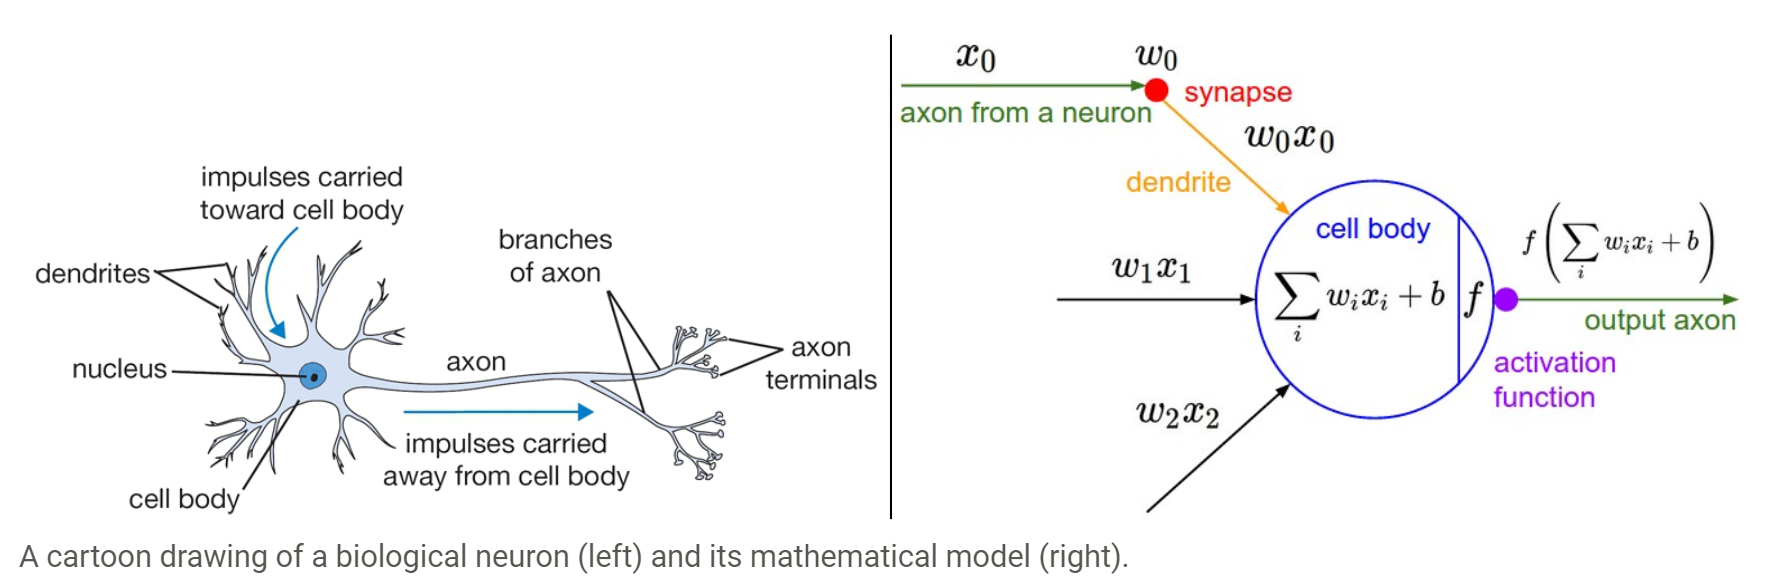
\includegraphics[width=0.9\linewidth]{fig/neuron_model.png}
\caption{\href{http://cs231n.github.io/neural-networks-1/}{神经元}(neuron)}
\end{figure}

常见的激活函数:
\begin{itemize}
    \item Sigmoid:$g(x)=\frac{1}{1+\ee^{-x}}$
    \item Tanh:$g(x)=\tanh(x)=\frac{\ee^{x}-\ee^{-x}}{\ee^{x}+\ee^{-x}}$
    \item ReLU:$g(x)=\max(0,x)$
\end{itemize}
之所以要采用非线性激活函数,是因为它可以使神经网络也变成非线性的,进而捕获到更加复杂的特征。

\begin{figure}[H]
\centering
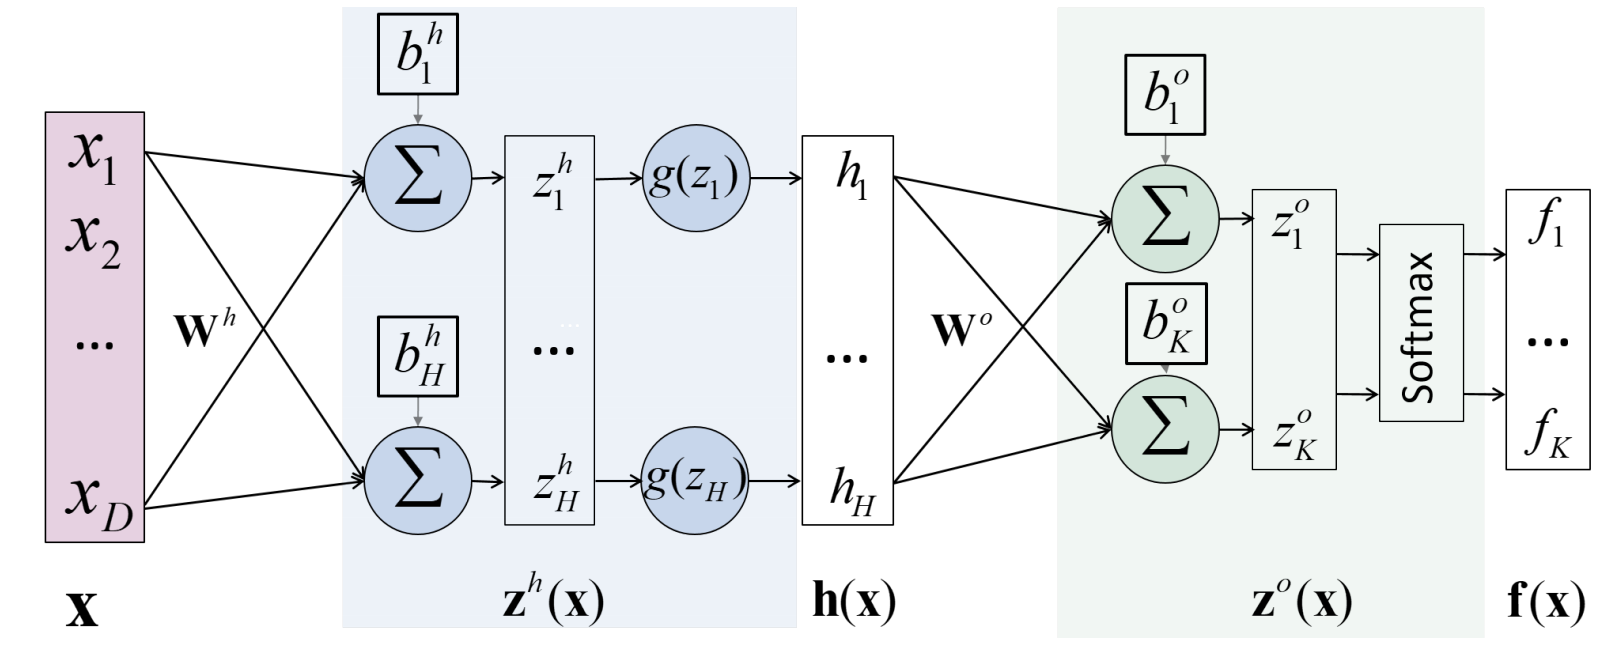
\includegraphics[width=0.8\linewidth]{fig/mlp.png}
\caption{多层神经网络(MLP)}
\end{figure}

但全连接层一个问题在于参数量巨大,当网络变大时计算量将爆炸,故要采用更加好的方法,既能提取出特征,同时计算量也能维持在一个合理的程度,因此就有了\newterm{卷积}(convolution)层。

\subsection{卷积}
$f$为原图,$g$为\newterm{卷积核}(kernel)或\newterm{滤波器}(filter)
\[(f*g)[i,j]=\sum_{m=-M}^M\sum_{n=-N}^Nf[i-m,j-n]g[m,n]\]
即对应元素相乘后相加(但注意卷积与相关操作的不同,\textemph{卷积要先取反})。
卷积在边界时可用0填充(padding)。

上面的公式只是2维卷积,现实我们训练的图片通常采用4维张量表示,即NCHW格式
\[\text{n\_samples}\times \text{n\_channels}\times \text{height}\times \text{width}\]
因此对于每一张多通道的图片,卷积核也应表示为3维,且确保卷积核通道数与图片的通道数相同,这样就可以在3维空间做卷积,但出来的图片只剩1个通道了。
故可以采用\textemph{$k$个权重不同}的卷积核\textemph{分别}对图片做卷积,那么就可以提取到$k$种不同的特征,出来的特征图(feature map)也会有$k$个通道。
% https://m2dsupsdlclass.github.io/lectures-labs/

在具体实施中,卷积层也是可训练的,卷积核的权重和偏置就可以通过网络学习得到。

卷积具有以下三个特征:
\begin{itemize}
    \item \textbf{稀疏交互}(sparse interactions):卷积层不像全连接层,是对整个图像进行权重计算,它只选择与卷积层交叠的部分进行计算。
    参数少了,自然计算量也少了。
    \item \textbf{参数共享}(parameter sharing):由于卷积核是滑过整个图片进行计算,因此对于卷积核的参数,都是被\textemph{多次}运用在不同位置的;而传统的全连接层的参数在图片的每一个位置只会被使用\textemph{一次},因此捕获细节特征的能力也会相对弱一些。
    \item \textbf{平移等变}(equivariant representation):哪怕图片进行一定的平移变换,卷积依然有办法将对应特征提取出来。
\end{itemize}

\bigskip
\begin{tcolorbox}
在图卷积神经网络(GCN)\cite{kipf:gcn_2017}中的卷积也是类似的道理,在一层中的所有图结点采用\textemph{相同}的神经网络进行聚集(aggregate)和更新(update)计算,这样子可以确保神经网络的参数共享,从而关注到图中的局部特征。
\end{tcolorbox}

\subsection{池化}
普通的小卷积只能捕获到低层的特征,想要获得高层的语义特征则卷积核应该有更大的\newterm{感受野}(receptive field),但大卷积又会使图片的细节部分被忽略。
为解决这两者之间的矛盾,可以在\textemph{缩小后的特征图做高层次的卷积}。
那么问题就变成了怎么缩小特征图,常见有两种方法:
\begin{itemize}
    \item 改变步长(stride)
    \item \newterm{池化}(pooling)/\newterm{降采样}(subsampling):对卷积核覆盖的范围取最值或平均
\end{itemize}

池化可以使得表示对于输入的微小变换保持近似不变(invariant),这也是好理解的,因为池化考虑的是一片区域的整体特征,对于取最值或是取平均来说,当局部区域一并改变时,池化后的结果确实不会有太多变化。

\bigskip
\begin{tcolorbox}
看到这好像也就能明白经典的LeNet为什么这么设计了。
先做卷积是为了提取图片中的小的/低层细节特征,然后做激活使得网络非线性,接着做池化,则是将图片进行缩放,方便后续的卷积提取出更大/更高层的语义特征。
\begin{figure}[H]
\centering
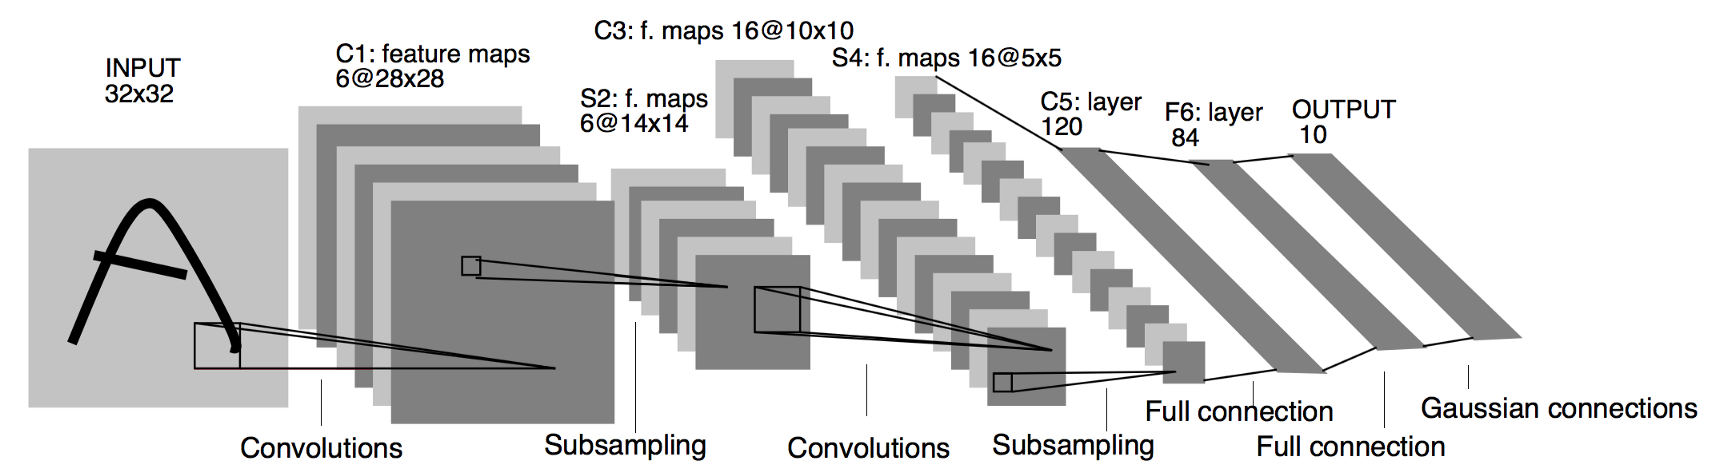
\includegraphics[width=\linewidth]{fig/lenet.png}
\caption{LeNet5}
\end{figure}
\end{tcolorbox}